\subsection{Ondas estacionárias na corda}

Como primeiro experimento, utilizaremos uma corda para poder estudar o comportamento de ondas estacionárias. Para atingir tal objetivo, utilizaremos um conjunto experimental que consiste de uma corda presa por um oscilador digital em uma das pontas e um peso na outra. Como o pesinho está passando por uma roldana, a força peso sele será transmitida e tracionará a corda.

\begin{figure}[H]
    \centering
    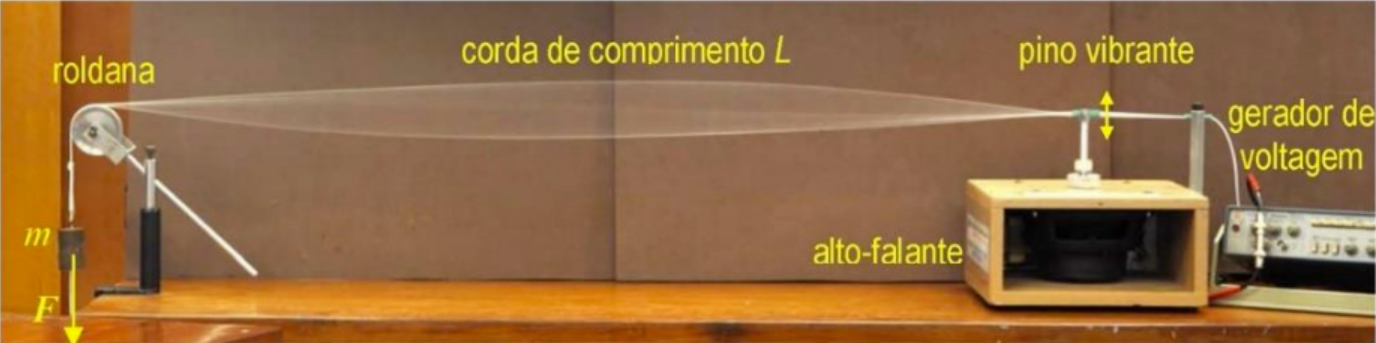
\includegraphics[width=0.8\textwidth]{images/montagem-ondas-corda.png}
    \caption{Montagem experimental para a Prática 1}
\end{figure}

Primeiramente nós vamos variar a frequência do oscilador para encontrar os 5 primeiros harmônicos da corda, que são as ondas estacionárias que nós queremos estudar. Anotaremos o valor da frequência ($f_n$; 1 $\leq$ n $\leq$ 5) quando aparecer. Com esses dados coletados nós podemos calcular o respectivo comprimento de onda para cada harmônico ($\lambda_n$) e assim encontrar a velocidade de cada onda ($v_n$). As fórmulas utilizadas serão:

\[ v_n = \lambda_n \cdot f_n \]
\[ \delta v_n = (\delta \lambda_n \cdot f_n) + (\lambda_n \cdot \delta f_n) \]

O valor de $\lambda_n$ é encontrado a partir da proporção entre o comprimento da corda ($L_c$) e o número do harmônico (n):

\[ \lambda_n = \frac{2 \cdot L_c}{n} \]
\[ \delta \lambda_n = \frac{2}{n} \cdot \delta L_c \]

Após determinar todas as 5 velocidades, faremos uma média simples:

\[ v_m = \frac{\sum_{n=1}^{5} v_n}{5} \]
\[ \delta v_m = \frac{\sum_{n=1}^{5} \delta v_m}{5} \]

E finalmente conseguiremos determinar a densidade linear experimental ($\mu_e$) da nossa corda em estudo utilizando a seguinte fórmula (note que a tração já foi substituída pela força peso):

\[ \mu_e = \frac{m_p \cdot g}{v_m^2} \]
\[ \delta \mu_e = \frac{(\delta m_p \cdot g \cdot v_m^2) + (m_p \cdot g \cdot 2 \cdot v_m \cdot \delta v_m)}{(v_m)^4} \]

Num segundo momento, vamos calcular diretamente a densidade linear ($\mu_d$) da corda utilizando o seu comprimento ($L_t$) e a sua massa ($m_c$), aplicando a seguinte relação:

\[ \mu_d = \frac{m_c}{L_t} \]
\[ \delta \mu_d = \frac{(\delta m_c \cdot L_t) + (m_c \cdot \delta L_t)}{(L_t)^2} \]

Assim sendo, teremos 2 parâmetros para comparar e podemos analisar se os nossos cálculos e equações foram deduzidos corretamente.
